\begin{frame}
\frametitle{Uniform Buffer: Demo}
\begin{figure}[ht]
    \centering
    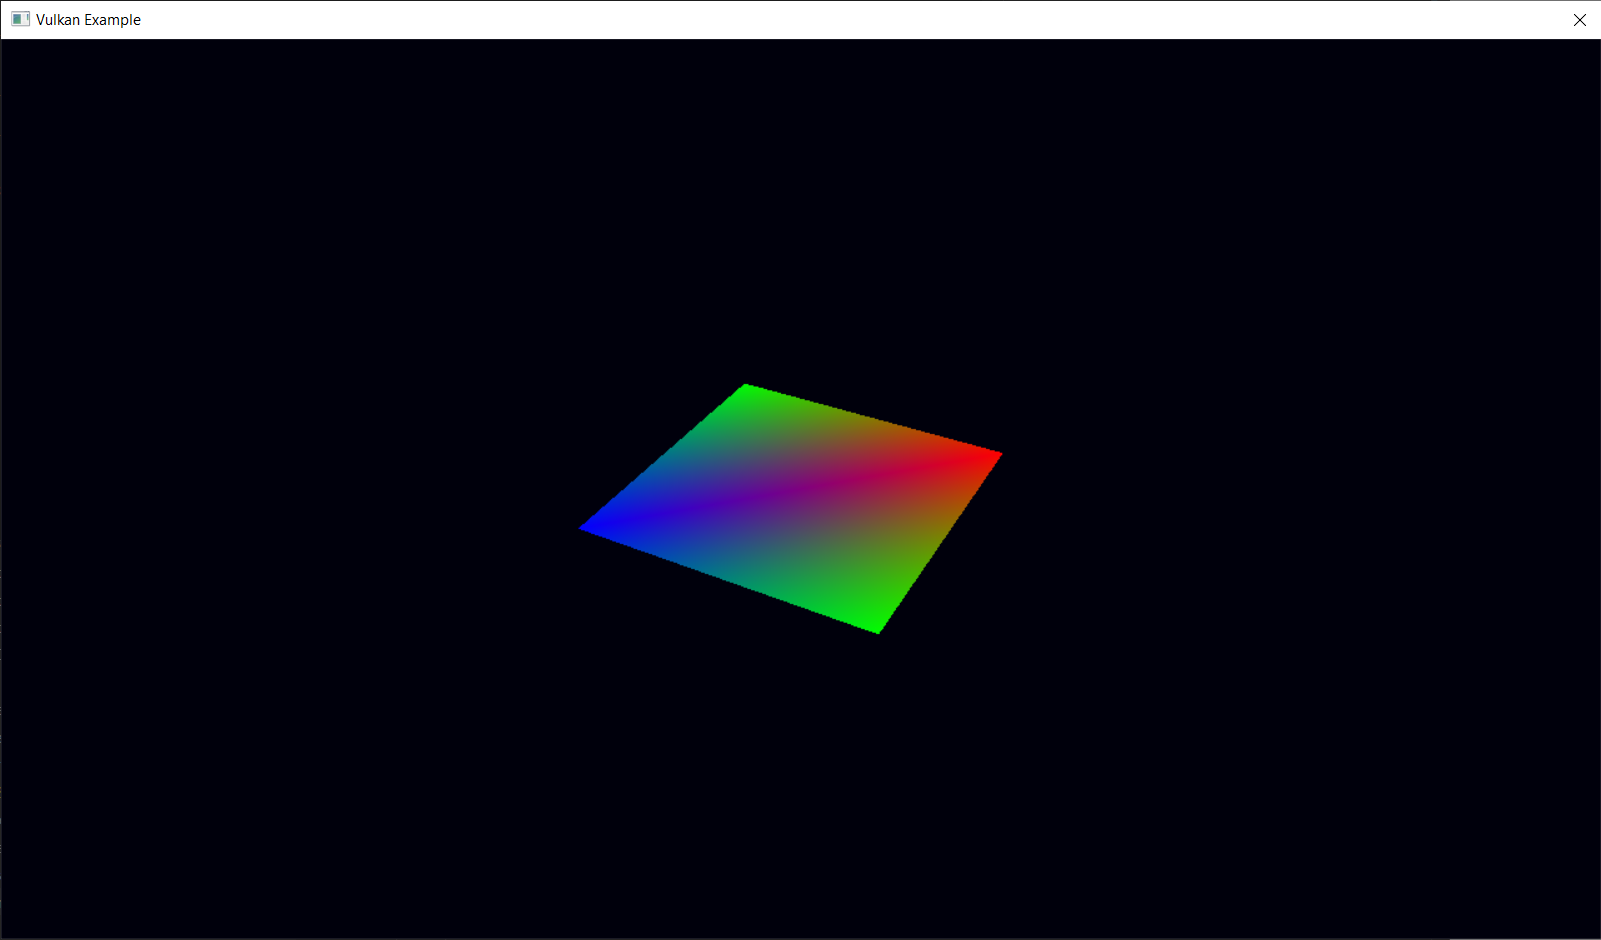
\includegraphics[scale=0.25]{images/SlidesUniforms/RenderQuad.png}
\end{figure}
\end{frame}

\begin{frame}
\frametitle{Uniform Buffer}
\begin{itemize}
\item Passiamo variabili globali agli shader usando uno uniform buffer
\item Siccome tali variabili cambiano frequentemente, allochiamo uno uniform buffer su memoria della GPU host visible
\item Informiamo di questo fatto la pipeline, usando un pipeline layout object
\item Tale oggetto descrive quali descriptor (risorse) sono globalmente accessibili in quali shader
\item Creiamo un descriptor set layout che descrive il numero e i tipi di descriptor
\item Allochiamo un descriptor set basandoci sul descriptor set layout
\item Una volta allocato, un descriptor set va popolato prima di essere utilizzato
\item Prima di scrivere il comando per attivare la pipeline, scriviamo nel command buffer un comando per informare la GPU che stiamo usando un certo descriptor set
\end{itemize}
\end{frame}
